\ProvidesFile{lecture10.tex}[Лекция 10]


\newpage
\section{Комплексные числа}

\subsection{Идея}

Почему нам вдруг не хватает вещественных чисел?
Давайте вспомним, а откуда получились вещественные числа?
Для начала у нас есть натуральные числа: $\mathbb N = \{1,2,3,\ldots\}$.
Которые мы беззаботно складывали и умножали.
Но как только нам захотелось посчитать $5 - 8$, как нам понадобились другие числа -- целые $\mathbb Z = \{\ldots, -2, -1,0,1,2,\ldots\}$.
И мы опять жили долго и счастливо, пока на не пришлось делить $2/3$ и тут пришлось построить рациональные числа $\mathbb Q = \{\frac{p}{q}\mid p,q\in \mathbb Z,\, q\neq 0\}$.
Вещественные нам пригодились, когда надо было решить уравнение $x^2 = 2$.
Тогда пришлось добавить $\sqrt{2}$, а заодно и кучу других полезных чисел.
Однако, этого опять оказалось мало и уравнение $x^2 +1 = 0$ не решается в вещественных числах.
При этом давайте заметим, что добавляя новые числа, операции над старыми мы не меняли.
Мы добавили целые, рациональные, вещественные, а натуральные как складывались и умножались по старым правилам, так и продолжают складываться и умножаться.

А какие-же числа мы хотим получить в идеале.
Прежде всего хочется решать уравнения вида $f(x) = 0$, где $f\in \mathbb R[x]$, всегда, когда это возможно.
Например, если $f = 1$, то решить такое уравнение по понятным причинам не возможно, но вот если $\deg f > 0$, то очень хочется иметь решение.
Новые числа должны содержать все вещественные как подмножество.
Но кроме этого, мы хотим уметь делать все арифметические операции с новыми числами, да еще так, чтобы старые операции не изменились.
И еще хочется по возможности быть экономными.
Вдруг, можно построить много разных лишних чисел (например, когда нам понадобились рациональные числа, мы могли по наивности и безрассудству сразу же построить вещественные, но обошлись более экономным вариантом в виде рациональных чисел).

Для того, чтобы формализовать идеи выше, нам надо строго сказать, а какой математической структурой должны являться новые числа.
Такими структурами являются поля.
Потом надо объяснить как правильно обращаться с полями, что с ними можно делать, как их сравнивать между собой.
И как только у нас появился зверинец полей, мы можем найти в нем поле комплексных чисел, как самое лучшее, которое только возможно среди тех, что удовлетворяют нашим запросам.


Сейчас нас ждет очередное абстрактное определение.
Напомню, что оно всегда состоит из двух частей: в первой части сказано какие у нас данные, а во второй -- каким аксиомам эти данные подчиняются.

\begin{definition}
[Поле]
Поле это следующий набор данных: $(F, + , \cdot)$, где
\begin{itemize}
\item $F$ -- некоторое множество.
Элементы этого множества называются числами.

\item $+\colon F\times F\to F$, $(x,y)\mapsto x+y$ -- некоторая операция называемая сложением.

\item $\cdot\colon F\times F\to F$, $(x,y)\mapsto xy$ -- некоторая операция называемая умножением.
\end{itemize}
Эти данные должны подчиняться следующим десяти аксиомам:
\begin{enumerate}
\item {\bf Ассоциативность сложения}
Для любых элементов $x,y,z\in F$ выполнено $x+(y+z) = (x+y)+z$.

\item {\bf Существования нейтрального по сложению}
Существует такой элемент $0\in F$ такой, что для любого $x\in F$ верно $x + 0 = 0 + x = x$.
Такой элемент называется нулем.

\item {\bf Существование обратного по сложению}
Для любого $x\in F$ существует элемент $-x\in F$ такой, что $x + (-x) = (-x) + x = 0$.
Такой элемент называется противоположным.

\item {\bf Коммутативность сложения}
Для любых элементов $x,y\in F$ верно $x+y = y+x$.

\item {\bf Ассоциативность умножения}
Для любых элементов $x,y,z\in F$ верно $x(yz) = (xy)z$.

\item {\bf Существование нейтрального по умножению}
Существует такой элемент $1\in F$, что для любого $x\in F$, верно $x 1 = 1 x = x$.
Такой элемент называется единицей.

\item {\bf Существование обратного по умножению}
Для любого элемента $x\in F\setminus\{0\}$ существует элемент $x^{-1}\in F$ такой, что $x x^{-1} = x^{-1}x = 1$.
Такой элемент называется обратным к $x$.

\item {\bf Коммутативность умножения}
Для любых элементов $x,y\in F$ верно $xy = yx$.

\item {\bf Дистрибутивность}
Для любых элементов $x,y,z\in F$ верно $x(y+z) = xy + xz$ и $(x+y)z = xz + yz$.

\item {\bf Нетривиальность}
$0\neq 1$.
\end{enumerate}
\end{definition}

\paragraph{Замечания}

Давайте сделаем несколько полезных замечаний.
\begin{enumerate}
\item Аксиомы сгруппированы следующим образом: (1--4) аксиомы на сложение, (5--8) аксиомы на умножение, (9) связь между сложением и умножением, (10) нетривиальность.
Причем аксиомы (1--4) и (5--8) идут по одному и тому же шаблону: ассоциативность, нейтральный элемент, обратный, коммутативность.
НО стоит отметить важную разницу между аксиомами (3) и (7).
По сложению обратный должен быть для любого элемента, по умножению только для ненулевого.
В частности, аксиому (7) нельзя сформулировать без аксиомы (2).

\item В аксиомах (2) и (6) не требуется единственность нуля и единицы.
Однако, можно показать, что если ноль существует, то он обязательно единственный, аналогично с единицей.
Действительно, если у нас есть два нуля $0_1$ и $0_2$, то рассмотрим их сумму $0_1 + 0_2$.
Так как $0_1$ является нулем, то $0_1 + 0_2 = 0_2$.
Так как $0_2$ является нулем, то $0_1 + 0_2 = 0_1$.
Значит оба нуля совпадают.
Аналогично проверяется единственность единицы.
Потому в силу однозначности эти элементы обозначаются $0$ и $1$.

\item В аксиомах (3) и (7) не требуется единственность обратного.
Однако, можно показать, что для любого $x$ существует единственный $-x$ и единственный $x^{-1}$.
Действительно, если для элемента $x\in F$ есть два элемента $y,z\in F$ таких, что
\[
x + y = y + x = 0\quad\text{и}\quad x + z = z + x = 0
\]
Тогда рассмотрим выражение
\[
(y + x) + z = y + (x + z)
\]
Его левая часть вычисляется в $0 + z = z$, а правая вычисляется в $y + 0  = y$.
А значит $y$ и $z$ совпадают.
То есть обратный по сложению будет один, аналогично с обратным по умножению.
Именно по причине однозначности им даются такие имена.
В частности однозначно определено число $-1$.

\item Мы привыкли к всяким замечательным свойствам, которым подчиняются числа $0$ и $1$.
Например: $x 0 = 0$ или $(-1)x = -x$ для любого $x$.
Оказывается, что их можно доказать пользуясь аксиомами.
Попробуйте сделать это.

\item Давайте рассмотрим множество $F=\{\cdot\}$ состоящее из одной точки.
Тогда на таком множестве существует единственная операция, положим сложение и умножение равными ей.
Тогда данный набор данных удовлетворяет всем аксиомам поля кроме последней.
Здесь ноль равен единице и вообще все элементы равны друг другу и ничего кроме  нуля (единицы) у нас  нет.
На самом деле, если ноль равен единице, то никаких других структур мы не построим.
Действительно, предположим $(F, +, \cdot)$ удовлетворяет всем аксиомам с первой по девятую, а вместо десятой -- ее отрицание $1 = 0$.
Тогда для любого элемента $a\in F$ имеем $a = a \cdot 1 = a \cdot 0$.
Давайте покажем, что $a \cdot 0 = 0$ для любого $a\in F$.
Рассмотрим равенство $0 + 0 = 0$, которое следует из определения нуля.
Умножим его на $a$, получим $a\cdot (0 + 0) = a \cdot 0$.
Раскроем скобки и получим $a \cdot 0 + a\cdot 0 = a\cdot 0$.
Теперь прибавим к обеим частям равенства элемент $- (a\cdot 0)$.
Получим
\[
a \cdot 0 + a\cdot 0 + - (a\cdot 0) = a\cdot 0 + - (a\cdot 0)
\]
Что равносильно $a\cdot 0 + 0 = 0$, а значит $a\cdot 0 = 0$, что и требовалось.
Потому последняя аксиома нужна для того, чтобы исключить именно этот дурацкий пример.
\end{enumerate}

\paragraph{Примеры}

Как только вам скормили абстрактное определение, первым делом нужны примеры.
Он помогут по-новому взглянуть на старых знакомых и разобраться с тем, а как вообще задавать эти самые новые объекты.

\begin{enumerate}
\item Рациональные и вещественные числа $\mathbb Q$ и $\mathbb R$ с обычными операциями.

\item Множество $\mathbb Q[\sqrt{2}] = \{a + b \sqrt{2}\mid a,b\in\mathbb Q\}\subseteq \mathbb R$ с обычными операциями является примером поля, которое лежит между $\mathbb Q$ и $\mathbb R$.

\item Рациональные функции $\mathbb R(x) = \{\frac{f}{g}\mid f,g\in\mathbb R[x]\}$.
Давайте думать про рациональные функции как про картинки.
Тогда на них определены формальные операции сложения и умножения.
Относительно этих операций они являются полем.

\item Теперь время экзотики $\mathbb F_2 =\{0, 1\}$, а операции берутся по модулю $2$.
Можно проверить, что и этот товарищ является полем.
Это очень важное поле для computer science.
Оно и его аналоги используются в теории кодирования, восстановления сигнала, архивирования и т.д.
\end{enumerate}



\begin{definition}
[Подполе]
Пусть $K$ и $L$ -- два поля причем $K \subseteq L$.
Тогда $K$ называется подполем в $L$, если операции сложения и умножения из $L$ ограниченные на $K$ дают сложение и умножение на $K$ соответственно.
Более подробно, пусть $+_L$ и $\cdot_L$ -- сложение и умножение на $L$, а $+_K$ и $\cdot_K$ -- сложение и умножение на $K$.
Тогда для любых элементов $x,y\in K$ верно: $x +_L y = x+_K y$ и $x\cdot_L y = x \cdot_K y$.
\end{definition}

По простому подполе -- это подмножество чисел в нашем поле, которое само является полем относительно операций из большего поля.
То есть нет никакой разницы какие операции использовать в подполе $K$: операции из $K$ или операции из $L$, так как между ними нет разницы.

\subsection{Абстрактное определение комплексных чисел}

\begin{definition}
Пусть поле $\mathbb C$ обладает следующими свойствами:
\begin{enumerate}
\item $\mathbb R\subseteq\mathbb C$ -- подполе, т.е. поле $\mathbb C$ содержит вещественные числа и операции сложения и умножения ограничиваются на $\mathbb R$ в обычные операции сложения и умножения.%
\footnote{В терминологии ниже вложение $\mathbb R\to \mathbb C$ является гомоморфизмом полей.}

\item Для любого не константного многочлена $f\in\mathbb C[x]$ существует корень $\alpha\in \mathbb C$, т.е. $f(\alpha) = 0$.

\item Поле $\mathbb C$ является минимальным полем, удовлетворяющим предыдущим свойствам, т.е. для любого поля $F$ такого, что $\mathbb R\subseteq F\subseteq \mathbb C$ если $F$ обладает двумя предыдущими свойствами, то $F = \mathbb C$.
\end{enumerate}
Тогда оно называется полем комплексных чисел.
\end{definition}

Стоит сделать важное замечание.
Из определения вообще говоря не следует, что подобное поле существует, но даже если оно и существует, то не понятно, вообще говоря, единственно ли оно.
Как можно ожидать, такое поле обязательно существует и оказывается, что оно единственно в некотором естественном смысле.
Потому идейно к определению выше надо относиться так: это набросок тех свойств, которые мы хотели бы получить от нашего поля, а дальше вся работа заключается в том, чтобы показать, во-первых, что таких свойств добиться можно и построить необходимое поле, а во-вторых, что как бы мы ни построили поле комплексных чисел, всегда получится одно и то же.

Как вы понимаете построить поле удовлетворяющее свойству (2) -- не простая задача.
Потому обычно поступают по-другому.
Мы построим поле с более слабым свойством, что существует решение только у уравнения $x^2 + 1 = 0$.
А уже потом покажем, что подобное поле удовлетворяет более сильному условию (2) из определения.
Единственность мы с вами доказывать не будем в силу того, что эта тема будет затронута в курсе алгебры в общем виде.

\subsection{Две модели комплексных чисел}
\label{subsection::ComplexModels}

В этом разделе я построю две модели комплексных чисел.
Для того чтобы различать эти модели, я для начала буду обозначать их $\mathbb C_1$ и $\mathbb C_2$.
Но как только мы поймем, что это одно и то же, мы будем опускать индекс и обозначать построенное поле через $\mathbb C$.

\paragraph{Символьная модель}

Пусть $\mathbb C_1$ -- это множество картинок вида $a+bi$, где $a,b\in\mathbb R$ -- вещественные числа, а $i$ и $+$ -- картинки.
Множество мы определили, теперь надо определить операции сложения и умножения.
Сумму картинок определим покомпонентно:
\[
(a+bi) + (c+di) = (a+c) + (b+d) i, \quad\text{где}\quad a,b,c,d\in\mathbb R
\]
Умножение определим исходя из соображений $i^2 = -1$.
Тогда
\[
(a+bi)(c+di) = (ac - bd) + (ad + bc)i,\quad\text{где}\quad a,b,c,d\in\mathbb R
\]
На этом этапе необходимые данные для определения поля нами построены.
Осталось дело за малым -- проверить все 10 аксиом.
Эту наинтереснейшую задачу я оставлю в качестве упражнения, но обязательно проверьте эти аксиомы.

Теперь $\mathbb C_1$ является полем.
Вещественные числа в него вкладываются так: число $r\in\mathbb R$ идет в картинку $r + 0 i\in\mathbb C_1$.
Теперь надо проверить, что сложить два вещественных числа -- это все равно, что сложить их как два комплексных числа.
Аналогично, умножить два вещественных числа -- это все равно, что умножить их как два комплексных числа.
Напоследок заметим, что комплексное число $i$ выбрано так, чтобы оно являлось решением уравнения $x^2 + 1 = 0$.

\paragraph{Матричная модель}

Пусть $\mathbb C_2$ -- это множество матриц вида $\left(\begin{smallmatrix}{a}&{-b}\\{b}&{a}\end{smallmatrix}\right)\in\Matrix{2}$.
Множество построено, теперь дело за операциями.
Придумывать их не надо, это будут обычные матричные сложение и умножение.
Единственное, что надо проверить, это что сумма и произведение матриц из $\mathbb C_2$ остаются в $\mathbb C_2$.%
\footnote{Это, пусть и легкое, упражнение мы оставляем на совести читателя.} 

Как и с первой моделью, мы только что построили все необходимые данные для определения поля, теперь надо проверить аксиомы.
И тут нам очень пригождаются матрицы.
Почти все аксиомы будут автоматически следовать из соответствующих свойств матричных операций.
Единственное, что надо проверить: коммутативность умножения и что любой ненулевой элемент обратим.
Я сейчас опять поступлю не очень честно и попрошу жаждущего знаний читателя все проверить самостоятельно.%
\footnote{На самом деле я всего лишь полу-честен с вами ибо чуть ниже будут проведены все соответствующие проверки.}

Вещественные числа вкладываются в $\mathbb C_2$ в виде скалярных матриц, то есть $r\in\mathbb R$ идет в $rE\in\mathbb C_2$.
Как мы знаем при этом операции матричного сложения и умножения превращаются в операции сложения и умножения вещественных чисел.
Осталось найти решение уравнения $x^2+1 = 0$.
Для этого заметим, что матрица $\left(\begin{smallmatrix}{0}&{-1}\\{1}&{0}\end{smallmatrix}\right)$ удовлетворяет этому уравнению.

\paragraph{Сравнение полей}

Для того чтобы сравнить различные поля и сказать, что они одинаковые или различные нам потребуется понятие изоморфизма полей.

\begin{definition}
Пусть $F_1$ и $F_2$ поля.
Отображение $\varphi\colon F_1\to F_2$ называется гомоморфизмом полей, если 
\begin{enumerate}
\item $\varphi(x+y) = \varphi(x) + \varphi(y)$ для любых $x,y\in F_1$.

\item $\varphi(xy) = \varphi(x)\varphi(y)$ для любых $x,y\in F_1$.

\item $\varphi(1) = 1$.
\end{enumerate}
Если $\varphi$ является биекцией, то оно называется изоморфизмом.
\end{definition}

Стоит отметить, что гомоморфизм полей всегда инъективен.
Попробуйте доказать это.
Кроме того, если отображение $\varphi$ инъективно, то достаточно лишь проверить первые два свойства гомоморфизма, т.е. единица автоматически перейдет в единицу.%
\footnote{Догадливый читатель уже сообразил, что в этом месте будет фраза: <<Проверьте это>>.}

Мы будем говорить что два поля изоморфны, если между ними существует изоморфизм.
Про изоморфные поля надо думать, как про одинаковые поля.
Действительно, что значит, что между множествами есть биекция.
Это значит, что это на самом деле одно и то же множество, а биекция лишь переопределяет имена, которыми называются наши элементы.
Изоморфизм кроме всего прочего сохраняет операции, это значит, что отождествив элементы наших полей, мы не различаем проделанных операций.
Так как поле для нас -- это множество с операциями, то значит мы не увидим никакой разницы, между полями, если в них одинаковые операции.

\begin{problems}
Пусть $\varphi\colon K\to L$ -- гомоморфизм полей.
Покажите, что выполнены следующие вещи:
\begin{enumerate}
\item $\varphi(0) = 0$.

\item $\varphi(-x) = -\varphi(x)$ для любого $x\in K$.

\item Если в определении гомоморфизма оставить только свойства $1$ и $2$, то $\varphi(1)$ либо $0$, либо $1$.
В частности, если $\varphi$ инъективно, то $\varphi(1) = 1$.

\item $\varphi(x^{-1}) = \varphi(x)^{-1}$ для любого ненулевого $x\in K$.
\end{enumerate}
\end{problems}

\paragraph{Сравнение моделей комплексных чисел}

Прежде чем объяснить, что $\mathbb C_1$ и $\mathbb C_2$ -- это одно и то же.
Нам понадобится еще одно определение.
Дело в том, что в наших полях лежат дополнительно вещественные числа и мы, когда будем сравнивать эти два поля, хотим чтобы это сравнение было согласовано в каком-то смысле с вещественными числами.

\begin{definition}
Пусть $F_1$ и $F_2$ -- два поля, содержащие поле вещественных чисел $\mathbb R$, то есть $\mathbb R\subseteq F_1$ и $\mathbb R\subseteq F_2$ и операции с $F_i$ ограничиваются на соответствующие операции на вещественных числах.
Будем говорить, что $\varphi\colon F_1\to F_2$ является изоморфизмом над $\mathbb R$, если 
\begin{enumerate}
\item $\varphi$ является изоморфизмом.

\item $\varphi(r) = r$ для любого вещественного числа $r\in \mathbb R$.
\end{enumerate}
\end{definition}

Давайте построим изоморфизм над $\mathbb R$ между $\mathbb C_1$ и $\mathbb C_2$.
А именно: $\varphi\colon \mathbb C_1\to \mathbb C_2$ будет действовать по правилу $a+bi \mapsto \left(\begin{smallmatrix}{a}&{-b}\\{b}&{a}\end{smallmatrix}\right)$.
По построению очевидно, что данное отображение является биекцией.
Кроме того, очевидно, что оно переводит сумму в сумму.
Методом пристального взгляда проверяем, что $\varphi$ сохраняет умножение.
Вещественное число $r = r + 0i$ переходит в матрицу $\left(\begin{smallmatrix}{r}&{0}\\{0}&{r}\end{smallmatrix}\right) = rE$.
С учетом нашего отождествления вещественных чисел с подмножествами в $\mathbb C_1$ и $\mathbb C_2$ последнее означает, что $\varphi(r) = r$ для любого $r\in\mathbb R$.
То есть нет никакой разницы между этими двумя моделями.
Причем на столько нет разницы, что при нашем отождествлении все новые числа в одной модели имеют ровно те же отношения со старыми числами, что и в другой (это по сути философия изоморфизма над $\mathbb R$).
С этого момента мы будем обозначать любую из этих двух моделей через $\mathbb C$.

\subsection{Простейшие свойства и операции}

\paragraph{Комплексное сопряжение}

Определим следующую операцию $\bar{\phantom{z}}\colon \mathbb C\to \mathbb C$ по правилу $z = a + bi \mapsto \bar z = a - bi$.
На языке матричной модели эта операция соответствует транспонированию.
Мы знаем, что транспонирование переводит сумму в сумму, а на произведении действует так $(AB)^t = B^t A^t$, но так как $\mathbb C_2$ коммутативно, то для матриц из $\mathbb C_2$ мы имеем $(AB)^t = A^t B^t$.
Кроме того сопряжение биективно, как видно из построения и переводит вещественные числа в вещественные.
Значит сопряжение является изоморфизмом $\mathbb C$ на $\mathbb C$ над $\mathbb R$.

Сделаем еще одно полезное замечание: на матричном языке сопряжение так же совпадает с вычислением присоединенной матрицы.
Действительно,
\[
\begin{pmatrix}
{a}&{-b}\\
{b}&{a}
\end{pmatrix}^t
= 
\begin{pmatrix}
{a}&{b}\\
{-b}&{a}
\end{pmatrix}
=
\widehat{
\begin{pmatrix}
{a}&{-b}\\
{b}&{a}
\end{pmatrix}}
\]

У последнего замечания есть интересное философское следствие.
Заметим, что сопряжение переводит $i$ в $-i$.
А так как оно является изоморфизмом, то это означает, что между $i$ и $-i$ нет никакой разницы.
То есть если мы внезапно обозначим $-i$ за $j$, то $i$ превратится в $-j$ и все комплексные числа будут иметь вид $a + bj$ и в этой новой форме никто не догадается, что $j$ это была $-i$, а не опечатка наборщика перепутавшего буквы $i$ и $j$.
То есть в поле комплексных чисел есть небольшая свобода выбора.
Мы случайно выбрали один из корней уравнения $x^2 + 1 = 0$ за $i$ и на самом деле нет никакой разницы какой из его корней мы так обозначим.

\paragraph{Вещественная и мнимая части}

Когда комплексное число записано в виде $z = a + bi$, где $a,b\in\mathbb R$, мы говорим, что это его алгебраическая форма.
В таком случае число $a$ называется его вещественной частью и обозначается $\Re z$, а $b$ называется мнимой частью $z$ и обозначается $\Im z$.
Числа с нулевой мнимой частью -- это вещественные числа, а числа с нулевой вещественной частью называются чисто мнимыми.

Заметим, что для любого числа $z\in\mathbb C$ верно
\begin{enumerate}
\item $z\in \mathbb R$ тогда и только тогда, когда $\bar z= z$.

\item $z\in i\mathbb R$ тогда и только тогда, когда $\bar z = - z$.
\end{enumerate}

\subsection{Геометрическая модель}

Комплексные числа $\mathbb C$ можно отождествить с вещественной плоскостью $\mathbb R^2$, а именно $a+bi$ соответствует вектору на плоскости $\left(\begin{smallmatrix}a\\b\end{smallmatrix}\right)$.
Таким образом про каждое комплексное число можно думать геометрически как про вектора.
При этом сложение комплексных чисел соответствует сложению векторов на плоскости.

У каждого вектора есть длина $|z| = \sqrt{a^2 + b^2}$ -- эта величина называется модулем комплексного числа.
В матричной модели у нас определитель, легко увидеть, что $\det z = |z|^2$.
Перечислим свойства модуля в следующем утверждении.

\begin{claim*}
Модуль комплексного числа обладает следующими свойствами:
\begin{enumerate}
\item $|{-}|\colon \mathbb C\to \mathbb R_+$ является нормой, то есть 
\begin{itemize}
\item $|z| \geqslant 0$ для любого $z\in\mathbb C$, причем равенство нулю достигается тогда и только тогда, когда $z = 0$.

\item $|\lambda z| = |\lambda | |z|$ для любого $\lambda \in \mathbb R$ и $z\in\mathbb C$.

\item $|z + w|\leqslant |z| + |w|$ для любых $z,w\in\mathbb C$.
\end{itemize}

\item $z\bar z = |z|^2$ для любого $z\in\mathbb C$.

\item $|zw| = |z| |w|$ для любых $z,w\in\mathbb C$.

\item $z^{-1} = \frac{\bar z}{|z|^2}$.
\end{enumerate}
\end{claim*}
\begin{proof}
Проверку (1) я оставлю на совести читателя.
(2) -- это явная формула.
(3) доказывается с использованием (2).
А вот (4) -- это явная формула для обратной матрицы, потому что в матричной модели $\bar z$ -- это сопряженная матрица, а $|z|^2$ -- это $\det (z)$.
\end{proof}

\paragraph{Тригонометрическая форма}

Пусть $z\in\mathbb C$ и пусть $z\neq 0$.
Тогда мы можем сделать следующее
\[
z = a + bi = \sqrt{a^2 + b^2}\left(\frac{a}{\sqrt{a^2 + b^2}} + \frac{b}{\sqrt{a^2 + b^2}}i\right)
\]
У числа в скобках вещественная и мнимая часть после возведения в квадрат в сумме дают единицу, а значит они являются косинусом и синусом некоторого числа $\varphi$, а значит, $z$ можно переписать в следующей форме
\[
z = |z| (\cos \varphi + i\sin\varphi)
\]
Такая запись комплексного числа называется тригонометрической.
Число $\varphi$ определено с точностью до $2\pi n$, $n\in\mathbb Z$ и называется аргументом комплексного числа.
Геометрически $\varphi$ -- это угол между осью $OX$ и вектором проходящим из нуля в $z$.
Угол отсчитывается против часовой стрелки.
Существует следующее удобное соглашение
\[
e^{i\varphi} = \cos \varphi + i \sin \varphi
\]
Оказывается, что при таком определении экспонента обладает всеми знакомыми нам свойствами.%
\footnote{Если заглянуть чуть глубже в большую науку, то окажется, что вас ждет некоторый набор чудес.
Окажется, что в комплексном мире очень мало гладких функций и они очень жесткие.
Это значит, что для любой вещественной гладкой функции $f\colon \mathbb R\to \mathbb R$ существует не более одной комплексной гладкой функции $\tilde f\colon \mathbb C\to \mathbb C$, продолжающей $f$, в том смысле, что $\tilde f(r) = f(r)$ для любой $r\in \mathbb R$.
Потому как бы мы не продолжили нашу вещественную экспоненту в комплексный мир, все эти способы дают одно и то же.}
В этом случае тригонометрическую форму можно записать так
\[
z = |z| e^{i\varphi} = e^{\ln |z| + i\varphi}
\]

Алгебраическая форма записи комплексного числа хорошо согласована со сложением, а тригонометрическая -- с умножением, о чем говорит следующее.

\begin{claim*}
Для комплексных чисел в тригонометрической форме верны следующие формулы
\begin{enumerate}
\item Пусть $z_1 = r_1(\cos \varphi + i \sin \varphi)$ и $z_2=r_2(\cos \psi + i \sin \psi)$ -- два ненулевых комплексных числа, тогда
\[
z_1 z_2 = r_1 r_2 (\cos(\varphi + \psi) + i\sin(\varphi + \psi))
\]

\item Пусть $z_1 = r_1(\cos \varphi + i \sin \varphi)$ и $z_2=r_2(\cos \psi + i \sin \psi)$ -- два ненулевых комплексных числа, тогда
\[
\frac{z_1}{z_2} = \frac{r_1}{r_2}(\cos(\varphi - \psi) + i\sin(\varphi - \psi))
\]

\item {\bf Формулы Муавра}
Пусть $z = r(\cos \varphi + i \sin \varphi)$ -- ненулевое комплексное число, тогда
\[
z^n = r^n (\cos(n \varphi) + i \sin(n \varphi))
\]
\end{enumerate}
\end{claim*}
\begin{proof}
1) По определению
\begin{gather*}
r_1(\cos \varphi + i \sin \varphi) r_2 (\cos \psi + i \sin \psi) = r_1 r_2 (\cos \varphi \cos \psi - \sin \varphi \sin \psi + i (\sin\varphi \cos \psi + \sin \psi \cos \varphi)) =\\ r_1r_2(\cos(\varphi + \psi) + i\sin (\varphi + \psi))
\end{gather*}

2) Можно проверить двумя способами.
Либо воспользоваться тем, что $1/z_2 = \bar z_2 /|z_2|^2$, либо домножить требуемое равенство на $z_2$ и тогда проверка сводится к первому пункту.

3) Это непосредственное следствие первого пункта.
\end{proof}

\subsection{Основная теорема алгебры}

\begin{definition}
Поле $F$ называется алгебраически замкнутым, если для любого многочлена $f\in F[x]\setminus F$ существует корень $\alpha\in F$, то есть $f(\alpha) = 0$.
\end{definition}

\begin{claim}
[Основная теорема алгебры]
\label{claim::CAlgClosed}
Поле $\mathbb C$ построенное в разделе~\ref{subsection::ComplexModels} алгебраически замкнуто.
\end{claim}

\paragraph{План доказательства}

Давайте я расскажу идейный план доказательства теоремы, чтобы у вас было понимание, что мы на самом деле будем делать ниже.
\begin{enumerate}
\item Рассмотрим произвольный не константный многочлен $p\in \mathbb C[x]$ и определим отображение $|p| \colon \mathbb C\to \mathbb R$ по правилу $z \mapsto |p(z)|$.
Первое что мы покажем, что это отображение достигает своего минимума в какой-то точке $z_0\in\mathbb C$.
Грубо говоря это будет следовать из того, что <<на бесконечности>> $|p(z)|$ стремится к бесконечности, а значит минимум может быть лишь <<возле нуля>>.
А <<возле нуля>>, то есть в каком-то диске содержащем ноль, функция $|p(z)|$ непрерывна, а потому достигает минимума.

\item Так как отображение $|p(z)|$ принимает только неотрицательные значения, то наличие нуля у многочлена $p$ равносильно тому, что в точке минимума $z_0$ значение $|p(z_0)|$ будет ноль.
Теперь надо будет показать, что минимум не может быть положительным.

\item Предположим, что минимум $r = |p(z_0)| \neq 0$.
Тогда значения $p(z)$ лежат вне диска радиуса $r$ с центром в нуле или на его границе.
Нам надо показать, что на самом деле если $r > 0$, то есть диск имеет внутренность, то у нас обязательно найдется значение $p$ внутри диска, что будет противоречить тому, что $z_0$ -- минимум $|p|$.
Последнее делается так: давайте выберем <<маленькую>> окружность вокруг точки $z_0$ и пройдемся по ней против часовой стрелки.
Тогда оказывается, что значения $p(z)$ пробегут по <<маленькой почти окружности>> вокруг $p(z_0)$ и может быть сделают более одного оборота.
А это значит, что обойдя вокруг $p(z_0)$, мы обязательно попадем внутрь диска радиуса $r$.
\begin{center}
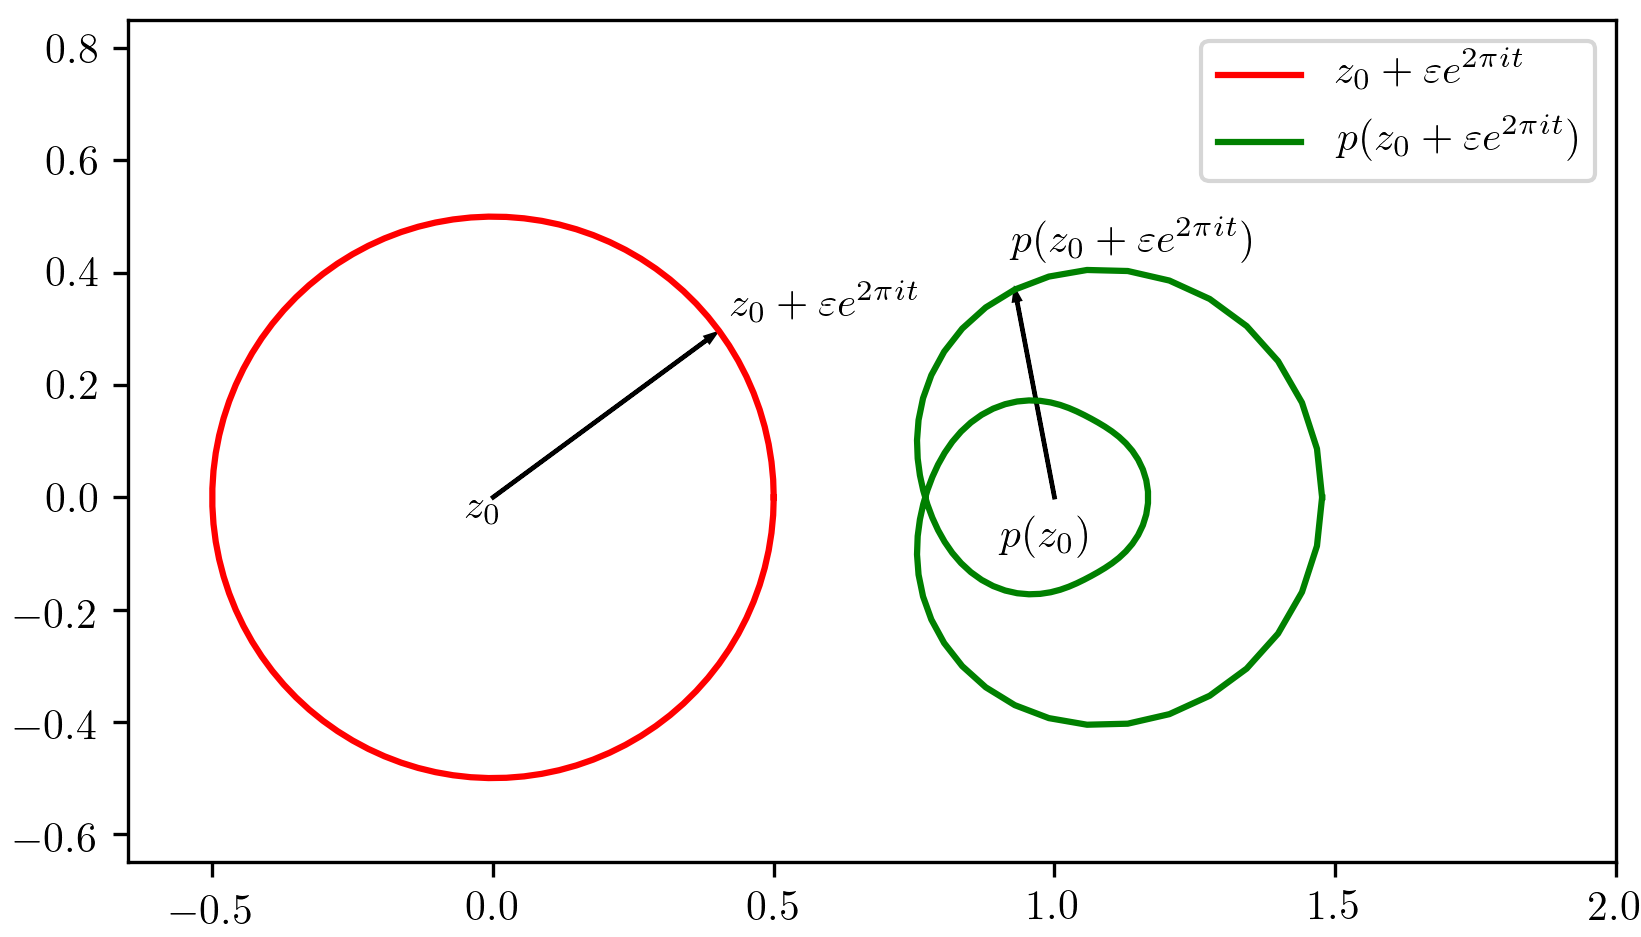
\includegraphics[scale = 0.5]{Figures/graph_cyrcle_cut.png}

Слева показана красным <<маленькая>> окружность вокруг $z_0$, а справа зеленым ее образ под действием $p$.
Здесь зеленая <<почти окружность>> делает два оборота.
\end{center}
\end{enumerate}
